\chapter{Introduction}
So far the best physical description of the universe is provided be the \ac{sm}.
But through observations of different phenomena, which the \ac{sm} can not explain, like neutrino oscillation \cite{} and the rotation velocity in galaxies \cite{}, it is known, that the \ac{sm} can not be a complete theory \cite{}.
Therefore different experiments are in developement or are operating to search for new physics and new particles outside the \ac{sm}.
One of these experiments is the proposed \ac{ship} experiment.
Some experiments are at the energy frontier, using large energy scale trying to discover new particles. The experiments at the \ac{lhc} are examples for energy frontier experiments.
Other experiments are at the cosmic frontieri, using for example cosmic background radiation.
The third frontier is the intensity frontier.
The zero background \ac{ship} experiment is one of the intensity frontier experiment searching for rare events.
Observing such rare events requires a high interaction rate.
To achieve this, \ac{ship} is planned to be a beam dump experiment at the \ac{sps} accelerator ring at CERN, as shown in \autoref{fig:sps_ship}.
The goal is to dump the high intensity \SI{400}{\giga\electronvolt} proton beam into a fixed target and thereby creating long lived particles outisde of the \ac{sm}, e.g. heavy neutral leptons and light supersymmetric particles \cite{ship}.
\begin{figure}
	\centering
	\includegraphics[width=0.75\textwidth]{pictures/ship_sps}
	\caption[Plan of the SPS area in which SHiP is supposed to be build.]{An overview of the SPS area with the SHiP experiment planed as beam dump experiment in the north area. \cite{ship_facility}}
	\label{fig:sps_ship}
\end{figure}

In \autoref{fig:ship_sketch} the overall struckture of \ac{ship} is shown.
At the beginning, the \SI{400}{\giga\electronvolt} gets dumped into the fixed targed.
Through the many interactions happening at the target, a lot of \ac{sm} particles will be created.
In order to block the \ac{sm} particles, two shields are placed after the target.
The first is a hadron absorber in which all \ac{sm} particles except muons and neutrinos are absorbed.
The second is the muon shield. 
It uses magnetic fields to deflect the muons away from the beam line.
The neutrinos cannot be blocked or deflected, but they are likely to be detected in the scattering and neutrino detector behind the muon shield.
After the neutrino detector a \SI{50}{\meter} long vacuum chamber is positioned.
If a non \ac{sm} particle is created at the target, is can decay inside the vacuum decay chamber back into \ac{sm} particles.
The decay products than get measured in the decay spectrometer behind the decay chamber.

One problem for the measurement are \ac{sm} particles entering the decay volume and causing events in the spectrometer.
An example of such a background are muons deflected by the muon shield but afterwrads reflected by the walls of the facility into to decay volume.
Therefore it is crucial for the zero background requirment to detect the particles entering the decay volume and tagging every event that could be caused by the entering particle as background.
For this the \ac{sbt} is in developement.
It is presented in the next chapter.



\begin{figure}
	\centering
	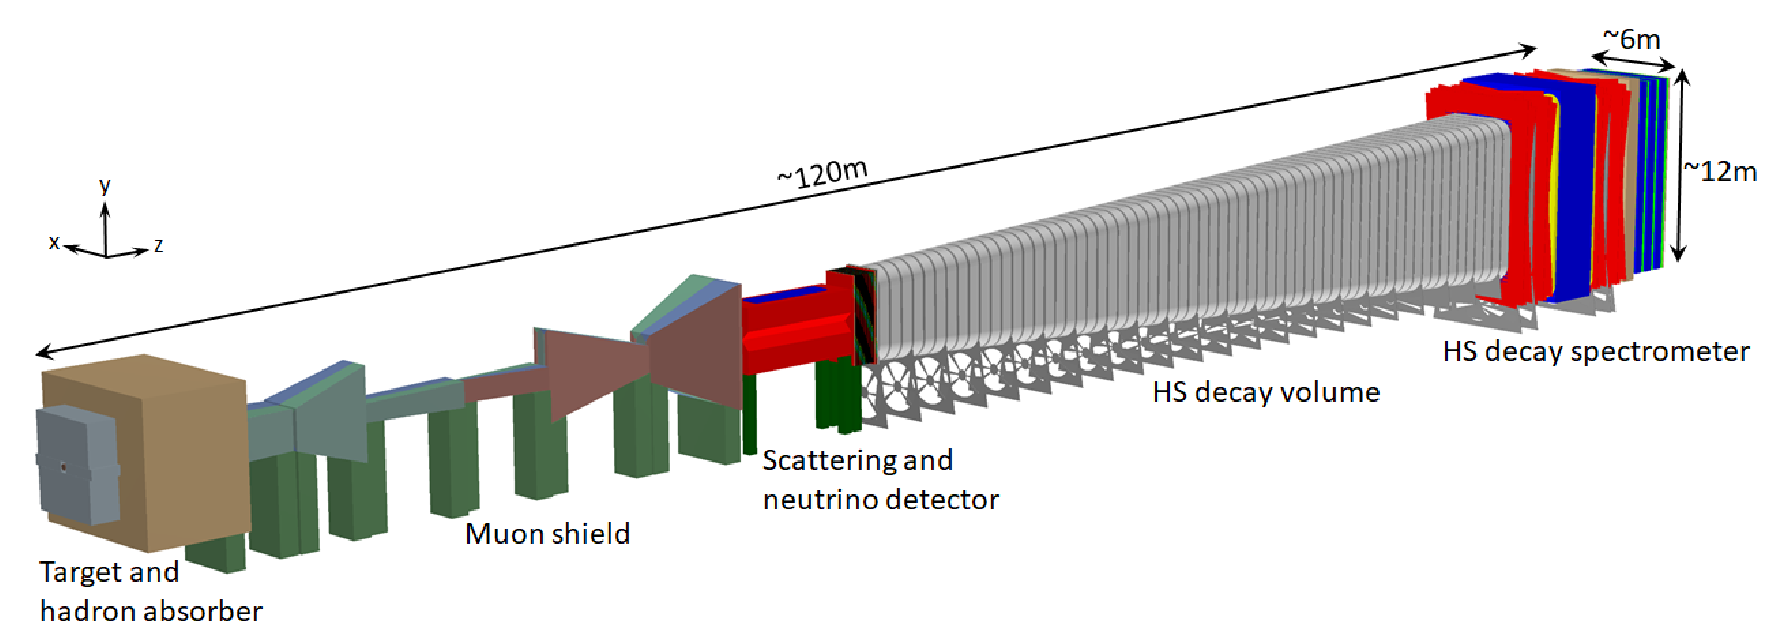
\includegraphics[width=1.\textwidth]{pictures/ship_sketch}
	\caption[Overview of the SHiP experiment.]{Overview of the proposed setup for the SHiP experiment. The target on the left is used as a beam dump for the SPS. Most standard model particles get absorbed by the hadron absorber directly behind the targed. A magnetic muon shield deflects the muon, which won't be absorbed by the hadron absorber, away from the beam line. After the muon shield is a scattering and neutrino detector and afterwards the \SI{50}{\meter} long decay volume in which non standard model particles created at the target can decay into standard model particles. To achieve the zero background goal, the Sourrund Background Tagger is around the decay volume. Behind the decay volume the decay spectrometer is placed. \cite{ship_coll}}
	\label{fig:ship_sketch}
\end{figure}
